% !TEX program = xelatex

% Nejlepší zážitek zaručí:
%
% TeX distribuce: texlive-full
%
% Editor:
%   VS Code s doplňky
%       * LaTeX Workshop
%       * LaTeX Utilities
%       * Gnuplot
%
% Další závislosti:
%   latexmk
%   bibtex
%   gnuplot


% Jak používat:
% Zkompilovat: make
% Gnuplot: make gnuplot
% Vyčistit: make clean


% Základní balíčky
\documentclass[10pt,a4paper]{article}
\usepackage[utf8]{inputenc}
\usepackage[czech]{babel}
\usepackage{graphicx}
\usepackage{wrapfig}
\usepackage{nonfloat}
\usepackage{lmodern}
\usepackage{amsmath}
\usepackage{hyperref}
\usepackage{gensymb}
\usepackage[top = 1cm, bottom = 1cm, left = 1cm, right = 1cm]{geometry}

% Bibtex
\usepackage{etoolbox}
\patchcmd{\thebibliography}{\section*{\refname}}{}{}{}

% Pro titulní stránku
\usepackage{titlesec}
\usepackage{setspace}
\usepackage{framed}
\usepackage{array}

% Vlastní balíčky
\usepackage{gnuplottex}
\usepackage{epstopdf}
\usepackage{csvsimple}
\usepackage{units}


\renewcommand{\U}[1]{\ensuremath{\,\mathrm{#1}}}
\newcommand{\°}{\degree}

\newcommand{\titjmeno}{Michal Grňo}
\newcommand{\titobor}{FOF}


\newcommand{\titcislo}{A21}
\newcommand{\titnazev}{Studium rentgenových spekter}
\newcommand{\titmereni}{11. 11. 2019}
\newcommand{\titodevzdani}{17. 11. 2019}


\begin{document}


\thispagestyle{empty}
\newgeometry{top = 2.5cm, bottom = 0cm, left = 2.5cm, right = 3cm}

{%T tomto je uzavřena celá titulka
%Tloušťka rámečku
\setlength{\fboxrule}{1.5pt}

\noindent
\framebox{
\begin{minipage}{\textwidth}
\setlength{\parindent}{17.62482 pt}
\phantom{d}

\begin{minipage}{0.6\textwidth}
{
\Large Kabinet výuky obecné fyziky, UK MFF\\
}
\vspace*{0.2cm}

{
\bfseries
\huge Fyzikální praktikum %ČÍSLO
}
\end{minipage}
\begin{minipage}{0.4\textwidth}
\begin{center}

\includegraphics[width=4.5cm]{ZFP.jpg}
\end{center}
\end{minipage}\\\\

%\vspace*{0.5cm}

{
\setstretch{1.5}
\Large
\noindent
Úloha č. \titcislo

\noindent
Název úlohy: \titnazev

\noindent
Jméno: \titjmeno
\hspace*{\fill}
Obor: \titobor

\noindent
Datum měření: \titmereni
\hspace*{\fill}
Datum odevzdání: \titodevzdani

\phantom{d}
}
\end{minipage}
}
%Konec horního rámečku

{
\phantom{d}

\Large
Připomínky opravujícího:\\
\vspace*{6.75cm}
}

\newcommand{\linka}{\noalign{\hrule height 1pt}}
\newcommand{\linkadva}{\noalign{\hrule height 1.5pt}}
\setlength\extrarowheight{9.5pt}
\Large
\noindent
\begin{tabular}{!{\vrule width 1.5pt} l !{\vrule width 1pt} c !{\vrule width 1pt} c !{\vrule width 1.5pt}}
\linkadva
   & Možný počet bodů & Udělený počet bodů \\\linkadva
  Práce při měření & 0-3 &  \\\linka
  Teoretická část & 0-2 &  \\\linka
  Výsledky a zpracování měření & 0-9 &  \\\linka
  Diskuse výsledků & 0-4 &  \\\linka
  Závěr & 0-1 &  \\\linka
  Použitá literatura & 0-1 &  \\\linkadva
  \hspace*{\fill} \textbf{Celkem} \hspace*{\fill}& max. 20 &  \\
\linkadva
\end{tabular}
\phantom{d}

Posuzoval: \hspace*{\fill}dne:~~~~~~~~~~~~~~~~~

}%Konec uzavření titulky
\newpage
\newgeometry{top = 2cm, bottom = 2cm, left = 2cm, right = 2cm}
\setcounter{page}{1}

\section{Pracovní úkoly}
\begin{enumerate}
    \item S využitím krystalu LiF jako analyzátoru proveďte měření následujících rentgenových spekter:
    \begin{enumerate}
        \item Rentgenka s Cu anodou.
        \begin{enumerate}
            \item proměřte krátkovlnné oblasti spekter brzdného záření při napětích 15 kV/1 mA, 25 kV/0,8 mA, 30 kV/0,8 mA, 33 kV/0,8 mA. K měření používejte tyto parametry: clonu o průměru 2 mm, interval Braggova úhlu pro 15 kV v rozmezí (10° – 15°) s krokem 0.2° a dobou expozice 8 s a pro ostatní napětí interval Braggova úhlu (3° – 10°) s krokem 0.2° a dobou expozice 5 s;
            \item proměřte charakteristická spektra rentgenky při napětích 15 kV/1 mA a 33 kV/0,8 mA. K měření používejte tyto parametry: clonu o průměru 2 mm, interval Braggova úhlu (15° – 30°), krok 0.1° a dobu expozice 2 s;
            \item proměřte tvar spektra s Zr absorbérem. K měření používejte tyto parametry: clonu s Zr absorbérem tloušťky 0.05 mm, interval Braggova úhlu (3° – 30°), krok 0.1° a dobu expozice 2 s;
            \item proměřte tvar spektra s Ni absorbérem. K měření používejte tyto parametry: clonu s Ni absorbérem tloušťky 0.01 mm, interval Braggova úhlu (3° – 30°), krok 0.1° a dobu expozice 2 s.
        \end{enumerate}
        \item Rentgenka s Fe anodou
        \begin{enumerate}
            \item proměřte charakteristické spektrum rentgenky při napětí 33 kV/0.8 mA. K měření používejte tyto parametry: clonu o průměru 2 mm, interval Braggova úhlu (3° – 30°), krok 0.1° a dobu expozice 2 s;
            \item proměřte tvar spektra s Zr absorbérem. K měření používejte tyto parametry: clonu s Zr absorbérem tloušťky 0.05 mm, interval Braggova úhlu (3° – 30°), krok 0.1° a dobu expozice 3 s.
        \end{enumerate}
        \item Rentgenka s Mo anodou.
        \begin{enumerate}
            \item proměřte charakteristické spektrum rentgenky při napětí 33 kV/0.8 mA. K měření používejte tyto parametry: clonu o průměru 2  mm, interval Braggova úhlu (3° – 35°), krok 0.1° a dobu expozice 3 s.
        \end{enumerate}
        \item Rentgenka s Cu anodou:
        \begin{enumerate}
            \item proměřte charakteristické spektrum rentgenky při napětí 33 kV/0.8 mA v intervalu Braggova úhlu (42° – 51°). K měření používejte tyto parametry: clonu o průměru 2 mm, krok 0.1° a dobou expozice 2 s.
        \end{enumerate}
    \end{enumerate}
    \item Interpretujte naměřené výsledky (pro mezirovinnou vzdálenost krystalu LiF používejte hodnotu d = 201,4 pm):
    \begin{enumerate}
        \item Krátkovlnná mez brzdného záření
        \begin{enumerate}
            \item Ze změřených mezních vlnových délek (respektive frekvencí) určete hodnotu Planckovy konstanty a oceňte přesnost měření
        \end{enumerate}
        \item Moseleyův zákon
        \begin{enumerate}
            \item Přesvědčte se, že naměřené úhlové frekvence spektrálních čar $K_\alpha$ a $K_\beta$ pro různé prvky splňují Moseleyův zákon. Ze směrnice příslušné závislosti určete hodnotu Rydbergovy úhlové frekvence a využitím této hodnoty určete též průměrnou hodnotu stínící konstanty.
            \item Přesvědčte se, že i naměřené polohy absorpčních hran Zr a Ni splňují Moseleyův zákon.
            \item Všimněte si, že absorpční hrana Ni koinciduje se spektrální čarou $K_\beta$ mědi; této skutečnosti se využívá v rentgenové difraktografii pro monochromatizaci charakteristického spektra mědi. Z provedeného měření určete filtrační efekt niklu pro čáru $K_\beta$.
        \end{enumerate}
        \item Úhlová disperze
        \begin{enumerate}
            \item Ze změřených spekter molybdenu určete velikost úhlové disperze pro různé řády difrakce.
        \end{enumerate}
    \end{enumerate}
\end{enumerate}

\pagebreak

\section{Teoretická část}
Rentgenka je zařízení, které vyzařuje rentgenové záření, pokud mu dodáváme dostatečné napětí. Je tvořena vakuovou baňkou, uvnitř které se nachází žhavená katoda, z níž vylétávají elektrony, a anoda, na kterou dopadají a při dopadu vyzařují elektromagnetické záření v rentgenové oblasti. Vznikající záření má dvě složky odpovídající dvěma různým způsobům, kterými vzniká. Jednak spojité brzdné záření, které vzniká když elektron prudce brzdí v elektromagnetickém poli anody. Toto záření není závislé na materiálu anody a nejvíce energetický foton, který dokáže při daném napětí vyprodukovat, má vlnovou délku $\lambda_m$, pro kterou platí
\begin{equation}
    eU = \frac{hc}{\lambda_m}.
    \label{mezni_lambda}
\end{equation}

My budeme provádět spektroskopii pomocí difrakce na mřížce LiF, vztah mezi měřeným úhlem a odpovídající vlnovou délkou udává tzv. Braggova rovnice:
\begin{equation}
    2d \sin \varphi = n\lambda,
    \label{bragg}
\end{equation}
kde $d=201.4 \U{pm}$ je mřížková konstanta LiF a $n$ je celé číslo udávající řád difrakčního maxima. Víme, že naměřený úhel v našem zařízení je zatížený aditivní chybou, z měření tedy budeme mít úhly $\vartheta$, pro které platí $\varphi = \vartheta + \vartheta_0$.

Budeme chtít pro ověření z naměřených dat vypočítat Planckovu konstatnu, vyjádříme si ji z rovnic~\eqref{mezni_lambda}~a~\eqref{bragg}, pro mezní úhel $\varphi_m$ potom bude platit:
\begin{align}
    h &= \frac{2eUd}{c} \frac{\sin \varphi_m}{n}, &
    \Delta h &= \frac{2eUd}{c} \frac{\cos \varphi_m}{n} \; \Delta\varphi
    \label{planck}
\end{align}


Druhý typ záření, který rentgenka produkuje, je tzv. charakteristické záření, které vzniká při excitaci a následné deexcitaci atomu anody. Toto záření je závislé na materiálu anody, úhlová frekvence fotonu odpovídající přechodu z $m$-tého excitovaného stavu do $n$-tého stavu je podle Rydbergova vztahu
\begin{equation}
    \omega = R_\omega (Z - s)^2 \left( \frac{1}{n^2} - \frac{1}{m^2} \right),
\end{equation}
kde $Z$ je atomové číslo prvku anody, $s$ je stínící konstanta a pro $R_\omega$ platí
\begin{equation}
    R_\omega = \frac{m_e e^4}{32 \pi^2 {\varepsilon_0}^2 \hbar^3}
    \approx  2.0606 \cdot 10^{16} \U{s^{-1}}
\end{equation}
Nás budou zajímat především spektrální čáry $K_\alpha$ a $K_\beta$, které odpovídají pádu z $m=2$, resp. $m=3$ do základního stavu $n=1$. Dosazením $m,n$ dostaneme tzv. Moseleyův zákon, který určuje vztah $\omega$ a $Z$:
\begin{align}
    \sqrt{\omega(K_\alpha)} &= \frac{\sqrt{3R_\omega}}{2}(Z-s),
    \label{omega-k-alpha} \\
    \sqrt{\omega(K_\beta)}  &= \frac{\sqrt{8R_\omega}}{3}(Z-s).
    \label{omega-k-beta}
\end{align}
Převedeme-li vlnovou délku v rovnici \eqref{bragg} na úhlovou frekvenci a dosadíme-li do předchozích rovnic, dostaneme lineární vztah:
\begin{align}
    \sqrt{\frac{n}{\sin\varphi(K_\alpha)}}
    = \frac{1}{2}\sqrt{ \frac{3R_\omega d}{\pi c} }(Z - s),
    \label{linearni-k-alpha} \\
    \sqrt{\frac{n}{\sin\varphi(K_\beta)}}
    = \frac{1}{3}\sqrt{ \frac{8R_\omega d}{\pi c} }(Z - s).
    \label{linearni-k-beta}
\end{align}
To jsou lineární vztahy tvaru $y = A(x - B)$, ze kterých můžeme lineární regresí zjistit stínící konstantu $s=B$ a Rydbergovu konstantu $R_\omega = \tfrac{4 \pi c}{3 d} A^2$, resp. $\tfrac{9 \pi c}{8 d} A^2$.

\pagebreak
\section{Výsledky měření}
\phantom{.}\vspace{-\baselineskip}
\begin{wrapfigure}{r}{8cm}
    \centering
    \vspace{-\baselineskip}
    \begin{gnuplot}[terminal=epslatex,terminaloptions={color size 8cm, 5cm}]
        set yrange [0:120]
        set key box opaque
        set key left width -10
        unset ytics

        set xlabel '$\vartheta [\°]$'
        set ylabel 'intenzita'

        n(x) = A*(x-B)
        f(x) = a*(x-b) + n(x)

        fit [0:8.35] n(x) 'data_Cu20kV-10s.dat' via A,B
        fit [8.35:8.8] f(x) 'data_Cu20kV-10s.dat' via a,b

        plot 'data_Cu20kV-10s.dat' t 'naměřená data', n(x) t 'šum (regrese)', f(x) t 'mezní chování (regrese)'

    \end{gnuplot}
    \vspace{-2\baselineskip}
    \caption{Způsob odečtu mezních úhlů, zde konkrétně u $^{29}$Cu při $20\U{kV}$.}

    \vspace{\baselineskip}

    \begin{gnuplot}[terminal=epslatex,terminaloptions={color size 8cm, 6.5cm}]

        set datafile separator ','
        load 'constants.cfg'

        LF_File = 'data_brzdne.csv'
        LF_Columns = 3
        load 'loadfile.cfg'

        N = LF_Rows - 1
        array U[N]
        array theta[N]
        array thetaerr[N]
        do for [i = 1:N] {
            U[i]        = LF_Col1[i+1]*1000
            theta[i]    = LF_Col2[i+1]
            thetaerr[i] = LF_Col3[i+1]
        }

        array h[N]
        array herr[N]
        do for [i = 1:N] {
            const = 2*e*U[i]*(d/c)
            h[i] = const * sin(theta[i]*deg)
            herr[i] = const * cos(theta[i]*deg) * thetaerr[i]*deg
        }

        set print 'data_planck.csv.tmp'
        print 'valU,valh,valherr'
        do for [i = 1:N] {
            print sprintf('%d,%f,%f', U[i]/1000, h[i]*1e34, herr[i]*1e34)
        }

        A = 1
        f(x) = A
        hh(x) = hh*1e34
        fit f(x) 'data_planck.csv.tmp' skip 1 using 1:2:3 yerrors via A

        set xrange [6:36]
        set yrange [5.8:7.1]
        set xlabel '$\theta [\°]$'
        set ylabel '$h [\U{10^{-34} J}]$'

        set key box opaque
        set key width -5

        plot sample [i=1:N] '+' using (U[i]/1000):(h[i]*1e34):(herr[i]*1e34) w yerrorbars t 'data', f(x) t 'vážený průměr', hh(x) t 'skutečná hodnota'

    \end{gnuplot}
    \vspace{-2\baselineskip}
    \caption{Naměřené hodnoty Planckovy konstanty}
    \label{graf-planck}

    \vspace{2\baselineskip}

    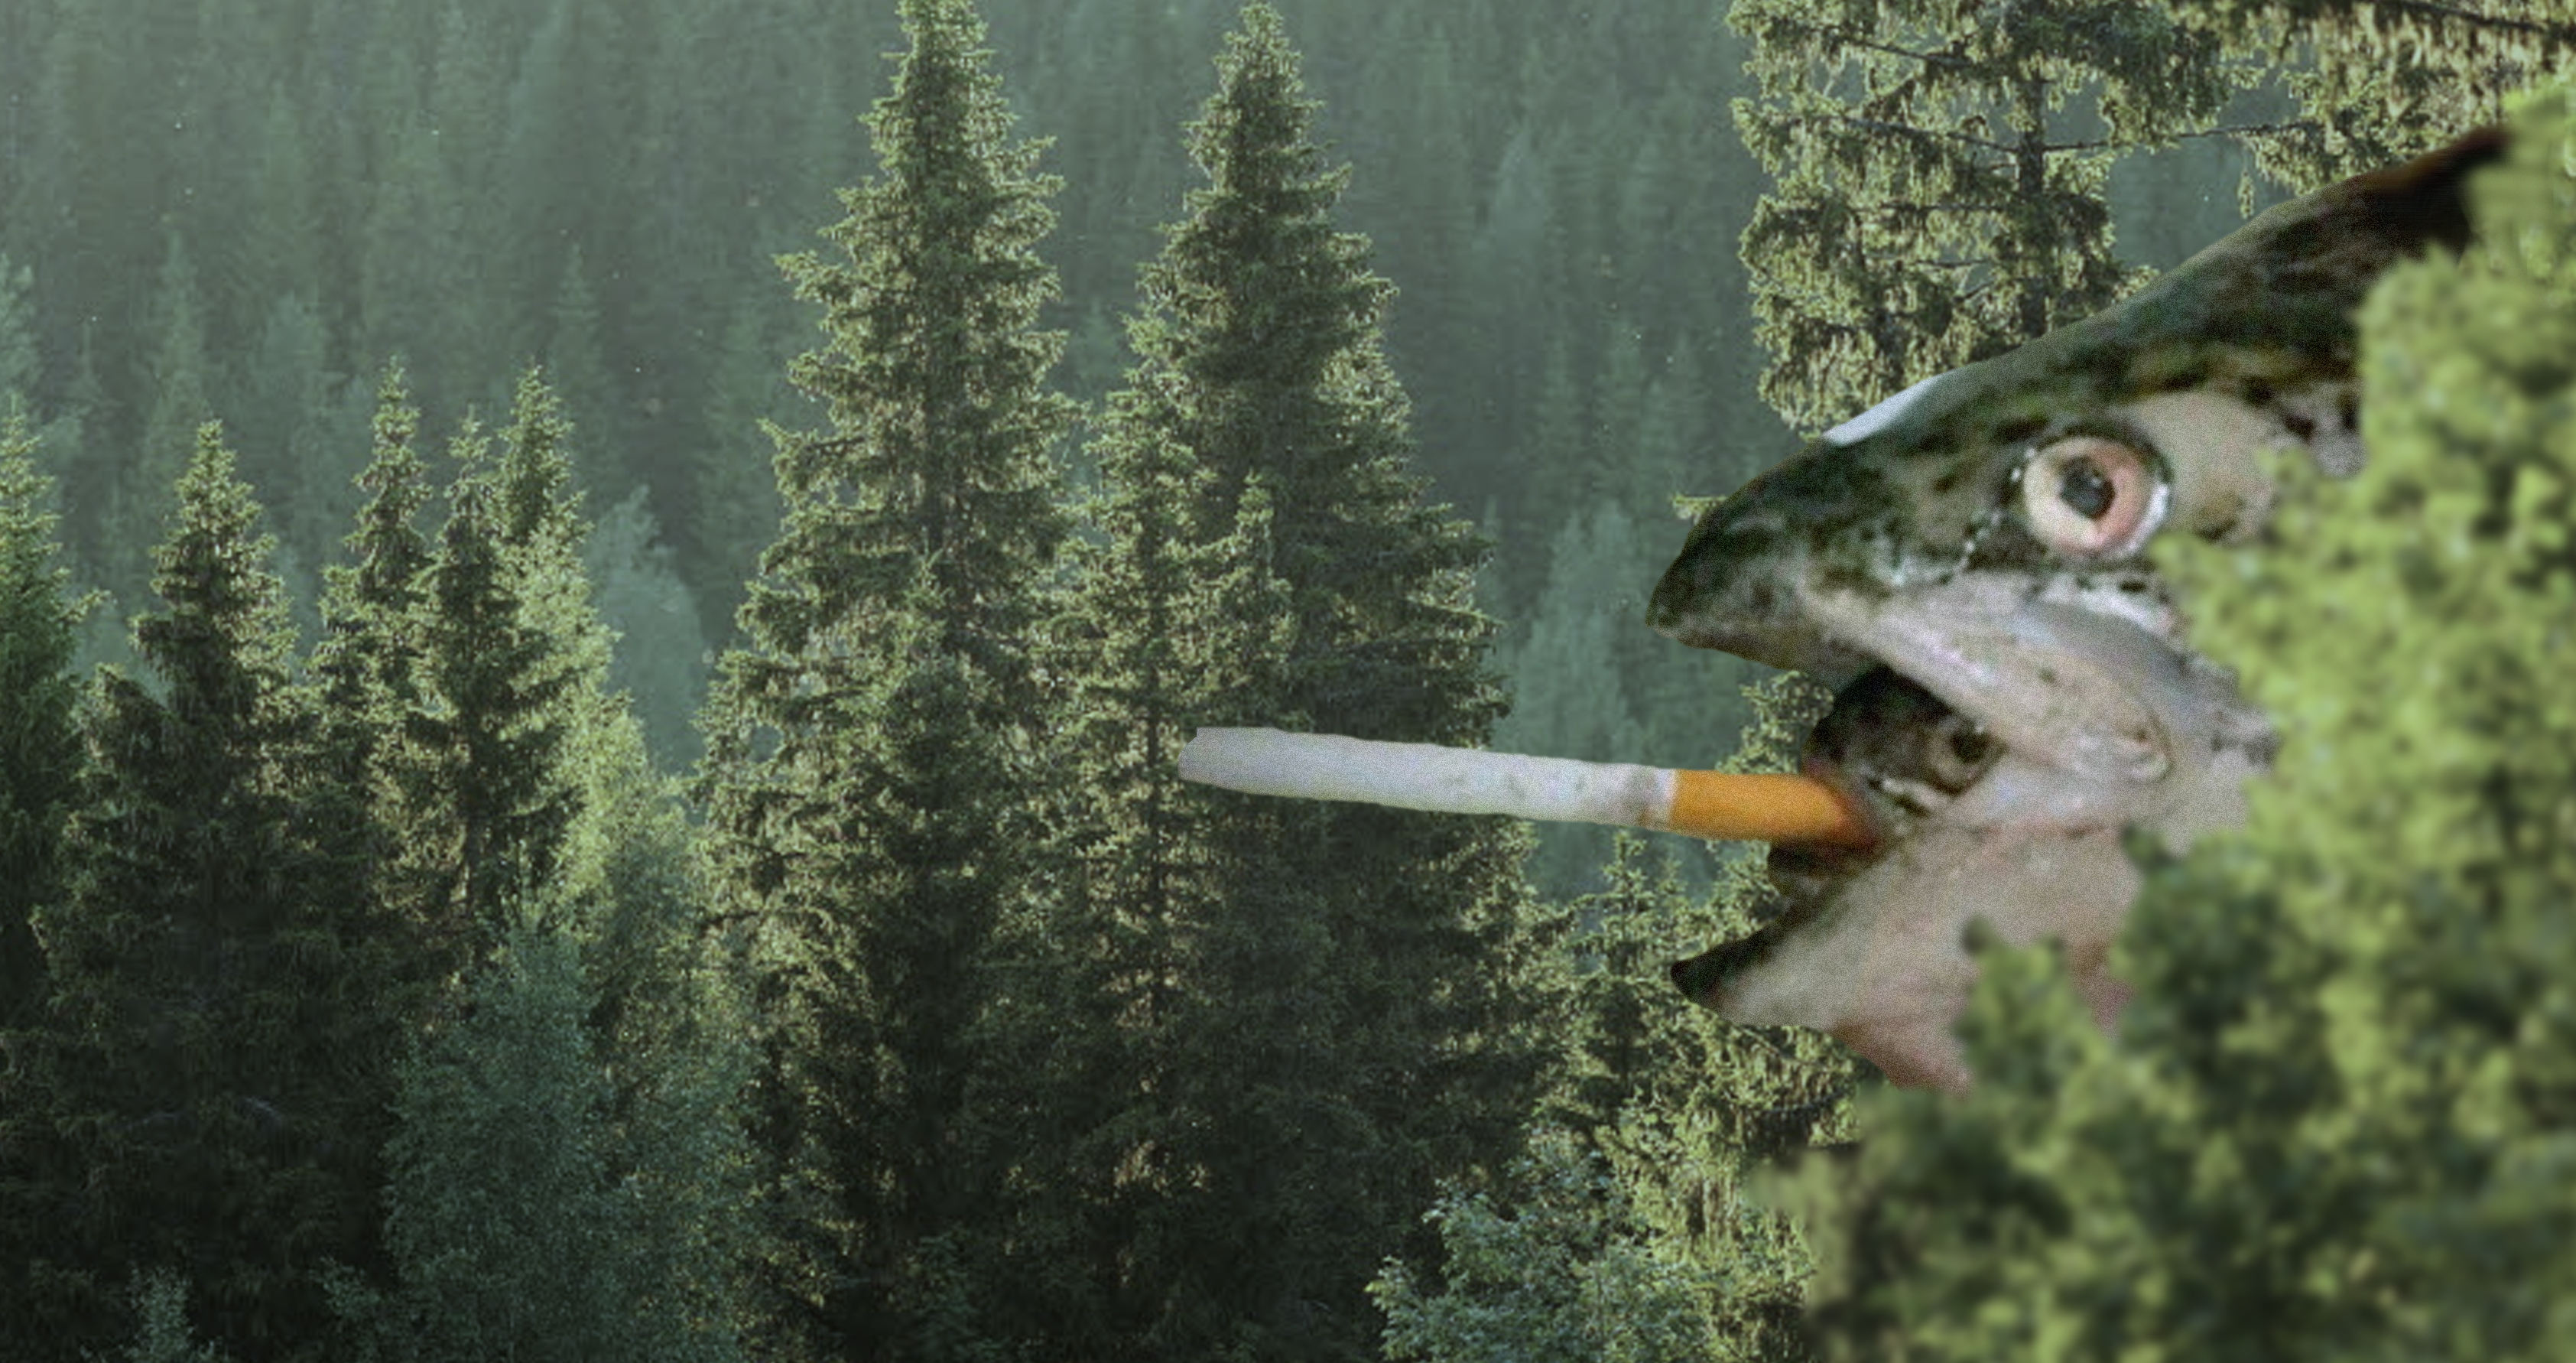
\includegraphics[width=7cm]{fish.jpeg}
    \vspace{-0.5\baselineskip}
    \caption{Pán lesa. Nepřeje si být rušen.}

    \vspace{2\baselineskip}

    \begin{gnuplot}[terminal=epslatex,terminaloptions={color size 8cm, 5cm}]

        set datafile separator ','
        load 'constants.cfg'

        LF_File = 'data_charakt.csv'
        LF_Columns = 6
        load 'loadfile.cfg'

        y(n, theta) = sqrt(n/sin(theta*deg + 0.55*deg))

        A = 1
        B = 1
        C = 1
        D = 1
        f(x) = A*(x-B)
        g(x) = C*(x-D)

        fit f(x) 'data_charakt.csv' skip 1 using 5:(y($1,$3)) via A,B
        fit g(x) 'data_charakt.csv' skip 1 using 5:(y($1,$4)) via C,D

        set key left top
        set xrange [24:44]
        set yrange [1.2:2.8]
        set xlabel '$Z$'
        set ylabel '$\sqrt{n/\sin\varphi}$'
        plot 'data_charakt.csv' skip 1 using 5:(y($1,$3)) title '$K_\alpha$' lc rgb 'red', 'data_charakt.csv' skip 1 using 5:(y($1,$4)) title '$K_\beta$' lc rgb 'blue', f(x) notitle lc rgb 'red', g(x) notitle lc rgb 'blue'

        set print 'fity.csv.tmp'
        print 'valA,valB,valC,valD'
        print sprintf('%.4f, %.4f, %.4f, %.4f', A, B, C, D)


        Ralpha = 4*pi*c/(3*d) * A**2 * 1e-16
        Rbeta = 9*pi*c/(8*d) * C**2 * 1e-16

        set print 'rydberg.csv.tmp'
        print 'valalpha, valbeta'
        print sprintf('%.4f, %.4f', Ralpha, Rbeta)
    \end{gnuplot}
    \vspace{-2\baselineskip}
    \caption{Lineární závislost z \eqref{linearni-k-alpha} a \eqref{linearni-k-beta}}
    \vspace{-13cm}
    \label{graf-linearni}
\end{wrapfigure}
Nejprve jsme měřili brzdné záření na rentgence s měděnou anodou. Extrapolací z grafů jsme určili mezní úhly:
\begin{minipage}{\linewidth}
    \vspace{\baselineskip}
    \centering
    \begin{tabular}{ r|rl }
        \bfseries $U [\U{kV}]$ &
        \multicolumn{2}{c}{$\vartheta [\°]$}
        \csvreader[ head to column names ]{data_brzdne.csv}{}
        {
            \csviffirstrow{\\\hline}{\\}
            \valU & \valtheta & $\pm$ \valthetaerr
        }
    \end{tabular}
    \vspace{\baselineskip}
    \tabcaption{Mezní úhly $\vartheta$}
    \label{mezni-uhly}
\end{minipage}

Autor připomíná, že $\vartheta$ značíme úhel ještě před korekcí na systematickou chybu. Úhel po korekci značíme ${\varphi = \vartheta + \vartheta_0}$.

Hodnoty Planckovy konstanty vypočtené podle \eqref{planck}, jejich průměř\footnote{Průměr je vážený převráceným čtvercem chyby.} a porovnání se skutečnou hodnotou je v grafu č. \ref{graf-planck}. Vidíme, že se skutečná hodnota signifikantně liší od té naměřené – to protože jsme zatím předpokládali, že systematická chyba $\vartheta_0 = 0$. Numericky nyní vyřešíme, pro jakou hodnotu $\vartheta_0$ se budou skutečná hodnota $h$ a vážený průměr rovnat. Získáme tím
\begin{equation}
    \vartheta_0 = 0.55 \°.
    \label{systematicka_chyba}
\end{equation}

Následně jsme měřili charakteristická spektra pro různé materiály anod. Pozorovali jsme maxima $n$-tého řádu na těchto úhlech:

\begin{minipage}{0.9\linewidth}
    \centering
    \vspace{\baselineskip}
    \begin{tabular}{ c|c|c|r|r }
        \multicolumn{1}{c|}{prvek} &
        \multicolumn{1}{c|}{$n$} &
        \multicolumn{1}{c|}{$U [\U{kV}]$} &
        \multicolumn{1}{c|}{$\theta(K_\alpha) [\°]$} &
        \multicolumn{1}{c}{$\theta(K_\beta) [\°]$}
        \csvreader[ head to column names ]{data_charakt.csv}{}
        {
            \csviffirstrow{\\\hline}{\\}
            $^{\valZ}$\prvek &
            \valn & \valU &
            \thetaalpha &
            \thetabeta
        }
    \end{tabular}
    \vspace{\baselineskip}
    \tabcaption{Úhly $\vartheta$ maxim charakteristického záření}
    \label{charakt-uhly}
\end{minipage}

Použitím hodnot z tabulky \ref{charakt-uhly} a vypočtené systematické chyby z \eqref{systematicka_chyba} jsme sestavili graf \ref{graf-linearni}. Podle Moseleyova zákona má být vztah mezi $Z$ a $\sqrt{n/\sin\varphi}$ lineární.

Proložením z grafu jsme získali parametry fitu
\csvreader[ head to column names ]{fity.csv.tmp}{}
{
    ${A(K_\alpha) = \valA}, \; {B(K_\alpha) = \valB}, \; {A(K_\beta) = \valC},$ ${B(K_\beta) = \valD}$
}. Z toho jsme vypočetli hodnoty Rydbergových konstant:
\begin{align*}
    \csvreader[ head to column names ]{rydberg.csv.tmp}{}
    {
        K_\alpha: \; R_\omega &= \valalpha \cdot 10^{16} \U{s^{-1}}\\
        K_\beta: \; R_\omega &= \valbeta \cdot 10^{16} \U{s^{-1}}
    }
\end{align*}

\pagebreak

\section{Diskuse}
Při měření se vyskytovala systematická chyba naměřeného úhlu. Ta byla korigována tak, aby $h$ vycházelo podle tabelovaných hodnot.

V grafu $I(\vartheta)$ závislosti intenzity na úhlu jsme pro velmi malé úhly pozorovali zesílení šumu – to bylo způsobeno faktem, že nemáme dokonale směrový zdroj ani detektor, detekovali jsme tedy záření, které nebylo difraktováno, ale doletělo do detektoru přímo. Pro vyšší úhly, tedy tam, kde jsme měřili hodnoty potřebné pro experiment, už tento jev neměl vliv.

Z grafu na obrázku č. \ref{graf-linearni} je vidět, že směrnice přechodů $K_\alpha$ a $K_\beta$ jsou jiné. To je pravděpodobně dáno tím, že Rydbergův vztah je pro všechny atomy, které nejsou vodík, pouze přibližný. I vypočtené hodnoty Rydbergovy konstatnty jsou kvůli tomu velmi odlišné pro $K_\alpha$ a $K_\beta$.


\section{Závěr}
Podařilo se vypočítat hodnotu Planckovy konstanty, jejím porovnáním se skutečnou hodnotou se podařilo určit systematickou chybu úhlu $\vartheta_0 = 0.55 \°$.

Podařilo se ověřit platnost Moseleyova zákona. Rydbergovy konstanty, které vyšly byly:
\begin{align*}
    \csvreader[ head to column names ]{rydberg.csv.tmp}{}
    {
        K_\alpha: \; R_\omega &= \valalpha \cdot 10^{16} \U{s^{-1}}\\
        K_\beta: \; R_\omega &= \valbeta \cdot 10^{16} \U{s^{-1}}
    }
\end{align*}
Jejich průměr je tedy $R_\omega = (2.1 \pm 0.5) \cdot 10^{16} \U{s^{-1}}$. Skutečná hodnota Rydbergovy konstanty je:
\begin{equation*}
    R_\omega = 2.0606 \cdot 10^{16} \U{s^{-1}}
\end{equation*}




\section{Literatura}
[1] Studijní texty k laboratorní úloze: Studium rentgenových spekter; Kolektiv autorů ZFP KVOF MFF UK, online zdroj, [cit. 8.11.2020], dostupné na stránkách fyzikálního praktika IV

\end{document}